% Course construction: shared source for print and native reference.
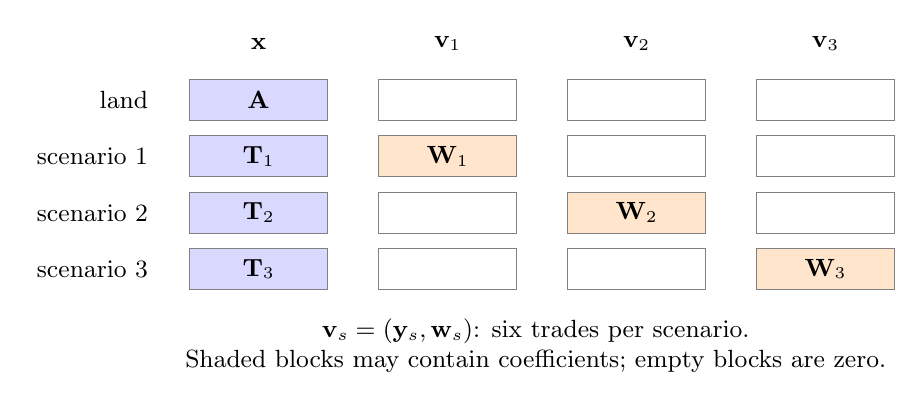
\begin{tikzpicture}[font=\small,x=.8cm,y=.65cm]
\foreach \x/\lab in {0/\mathbf{x},3/\mathbf{v}_1,6/\mathbf{v}_2,9/\mathbf{v}_3}
 \node at (\x+1.1,.7) {$\lab$};
\foreach \yy/\lab in {0/land,-1.1/scenario 1,-2.2/scenario 2,-3.3/scenario 3}
 \node[anchor=east] at (-.5,\yy-.4) {\lab};
\fill[blue!15] (0,0) rectangle (2.2,-.8);
\foreach \yy/\xx/\s in {-1.1/3/1,-2.2/6/2,-3.3/9/3}{
 \fill[blue!15] (0,\yy) rectangle (2.2,\yy-.8);
 \fill[orange!20] (\xx,\yy) rectangle (\xx+2.2,\yy-.8);
 \node at (1.1,\yy-.4) {$\mathbf{T}_{\s}$};
 \node at (\xx+1.1,\yy-.4) {$\mathbf{W}_{\s}$};
}
\node at (1.1,-.4) {$\mathbf{A}$};
\foreach \yy in {0,-1.1,-2.2,-3.3}
 \foreach \xx in {0,3,6,9}\draw[gray] (\xx,\yy) rectangle (\xx+2.2,\yy-.8);
\node[align=center] at (5.5,-5.2) {$\mathbf{v}_s=(\mathbf{y}_s,\mathbf{w}_s)$: six trades per scenario.\\Shaded blocks may contain coefficients; empty blocks are zero.};
\end{tikzpicture}
